In the last years, the storage capacity of hard disk drives has
increased dramatically while at the same time their price has
decreased. Even though solid-state drives are still quite expensive,
big enterprises may benefit from the throughput they provide. This
trend of ``cheap'' storage solutions has led companies and research
institutes to store a volume of data that has never been stored
before. In 2014 Facebook was processing 600 TB daily
\footnote{https://code.facebook.com/posts/229861827208629/scaling-the-facebook-data-warehouse-to-300-pb/}
while according to rough estimates
\footnote{https://what-if.xkcd.com/63/} around 15 exabytes are stored
in Google's datacenters.

Another interesting area that is already generating a huge volume of
raw data is the DNA sequencing. According to \cite{10.1371/journal.pbio.1002195} the Sequence
Read Archive maintained by the United States National Institutes of Health
National Center for Biotechnology Information already contains more
than 3.6 petabytes of raw sequence data for a wide variety of samples
including microbial genomes, plant and animal genomes and human
genomes. As we can see in Figure \ref{fig:intro_genomics_growth} the
need for storage capacity will exceed the order of PetaBytes by the
year 2025.

\begin{figure}
\centering
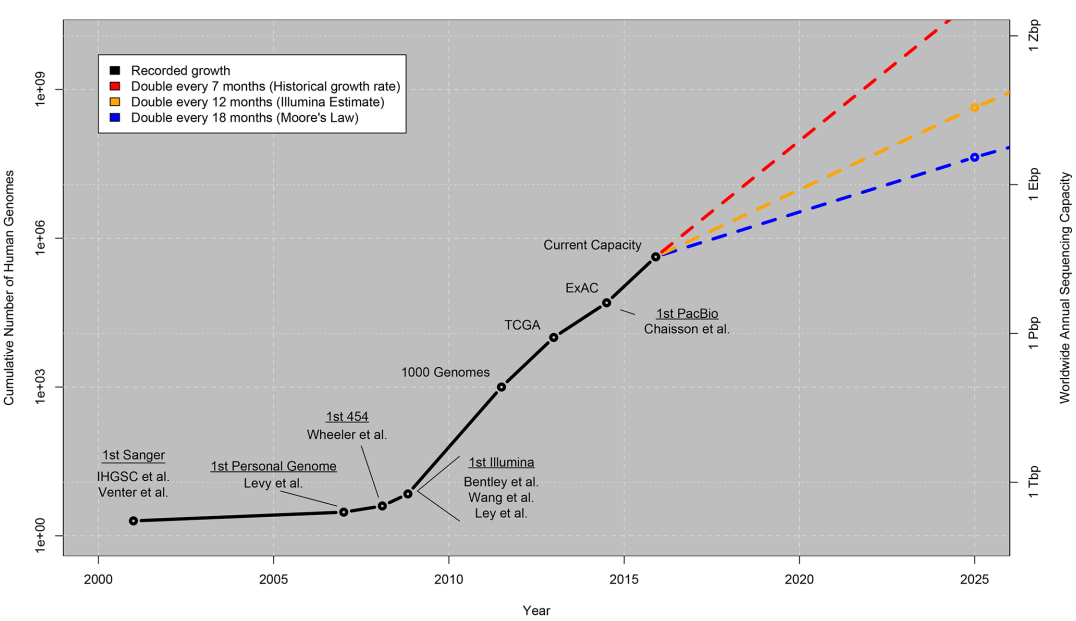
\includegraphics[scale=0.5]{resources/images/Introduction/genomics_growth.png}
\caption{Growth of DNA sequencing \cite{10.1371/journal.pbio.1002195}}
\label{fig:intro_genomics_growth}
\end{figure}

It is clear by now that these volumes need a paradigm shift
from the traditional way we store and analyze data. It is not possible
anymore to store them in a single machine. We need to employ a
distributed system to harness the power of those data and extract
valuable results within a reasonal time frame. On top of that we have
to take under consideration that hardware will fail for various
reasons. A minimum requirement would be not to lose our data, so we
should keep them in several replicas. Going one step further, we would
like our analyzing jobs to continue running even though one machine failed. These
jobs usually take hours to complete, so re-running them is not the
best approach.
